% !TEX root = ../main.tex
\iflatexml
\begin{figure}
    \centering
    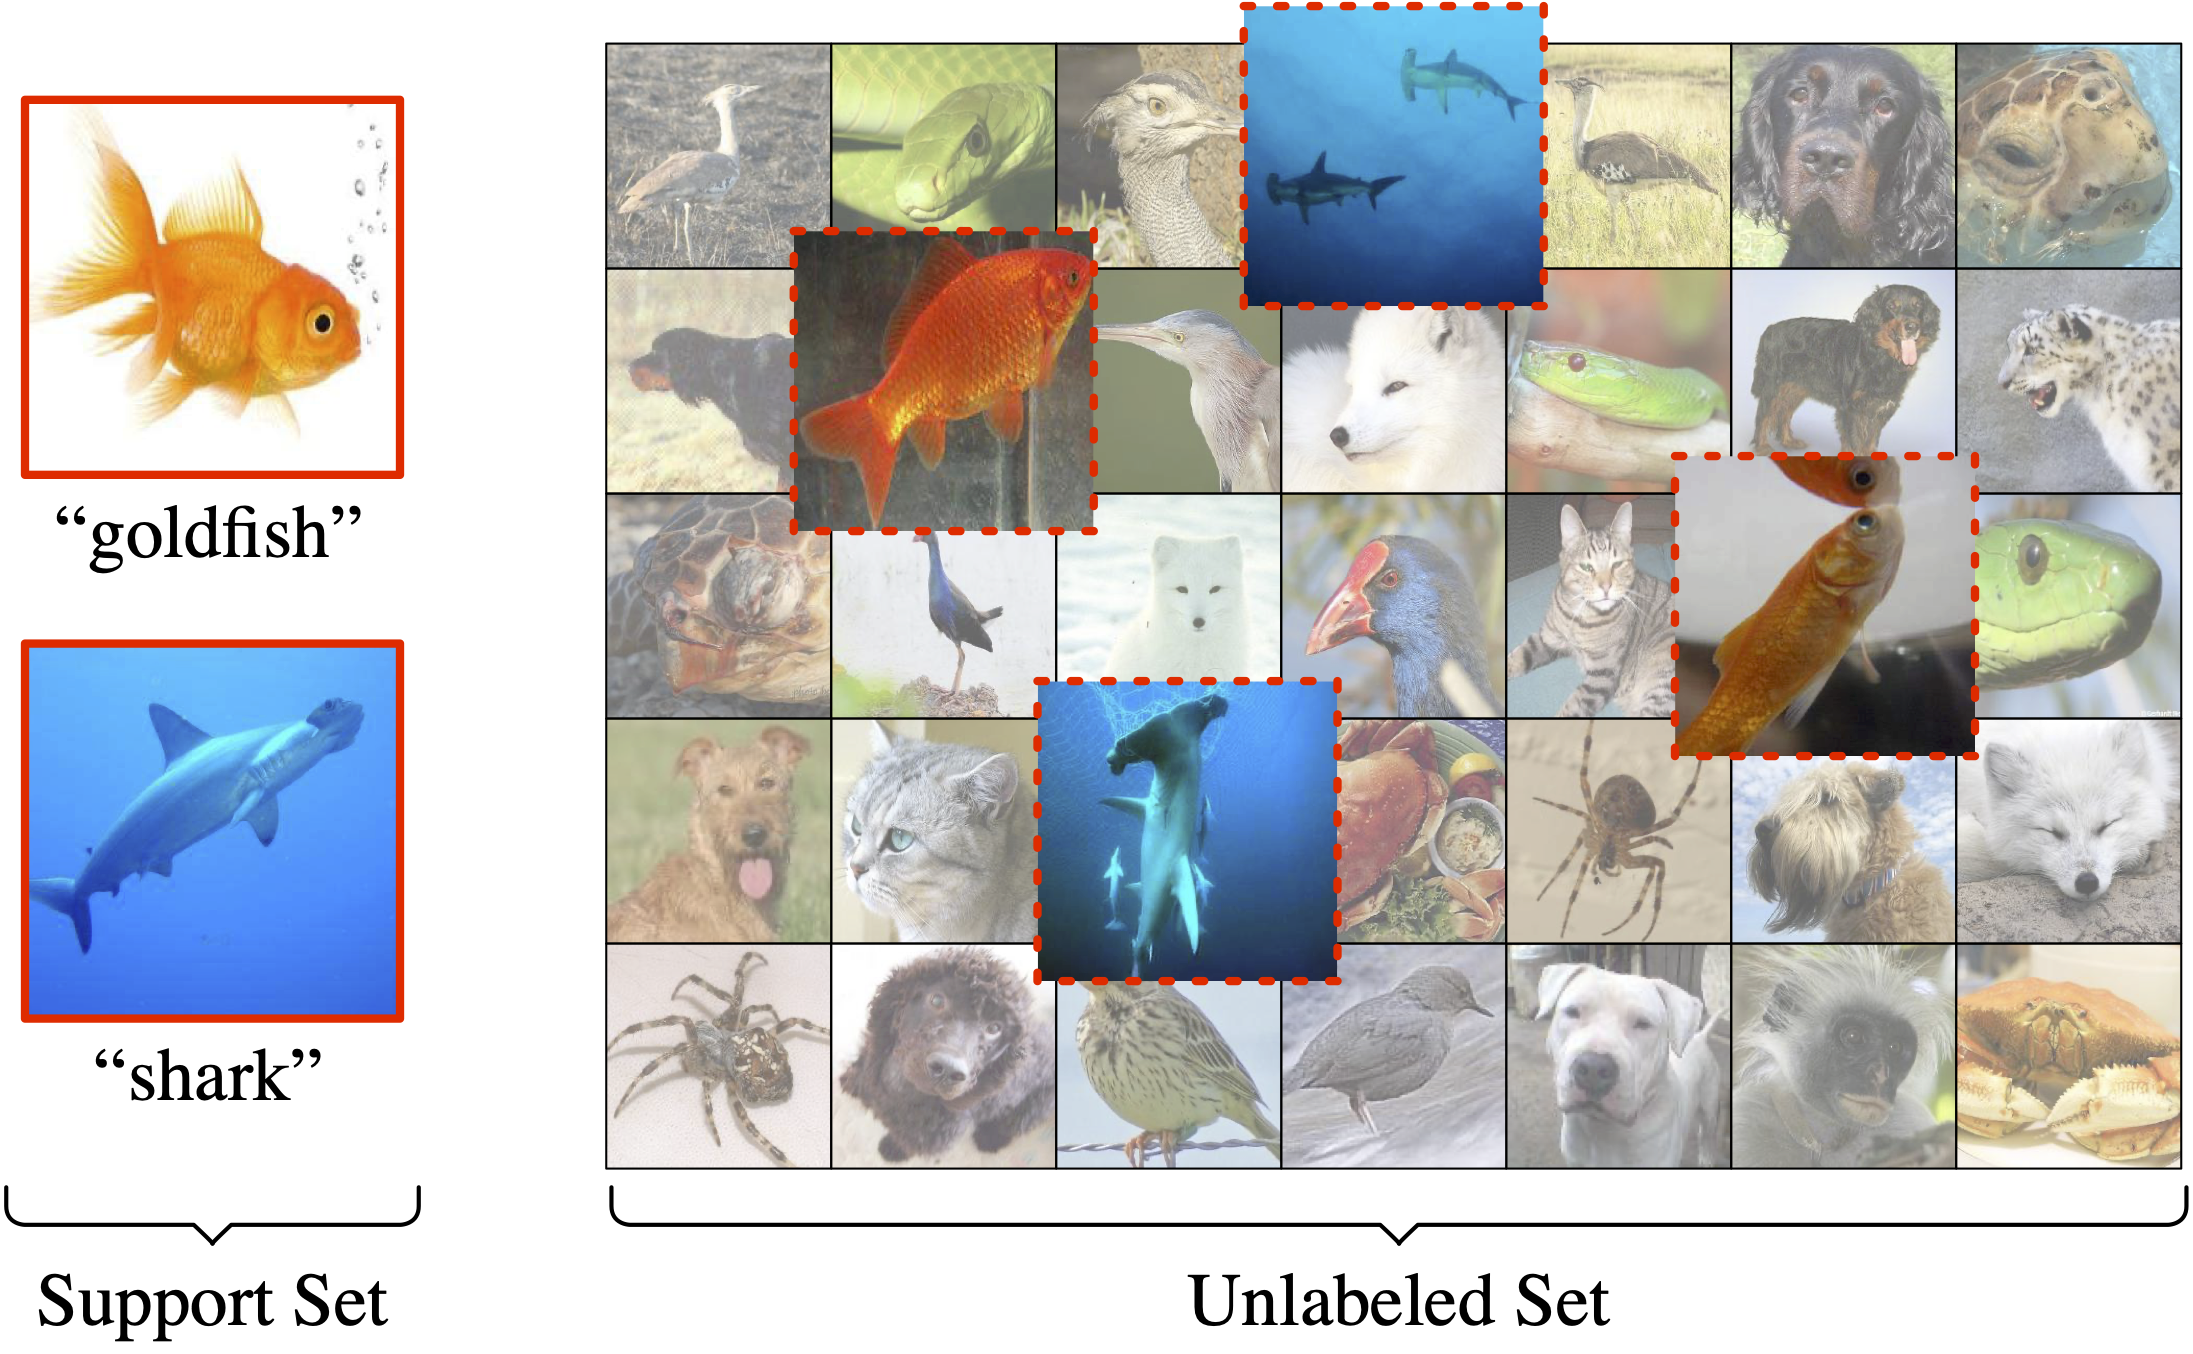
\includegraphics[width=6\textwidth]{figures/ssl_teaser_grid_distractor_fade_enlarge.png}
    \caption{Consider a setup where the aim is to learn a classifier to distinguish between two previously unseen classes, goldfish and shark, given not only labeled examples of these two classes, but also a larger pool of unlabeled examples, some of which may belong to one of these two classes of interest. %Specifically, we are exposed to a small number of labeled images for each of these two classes, denoted by a red border, and a larger number of unlabeled objects belonging to the classes of goldfish or shark, shown enlarged in this figure, as well as to ``background'' classes. 
    In this work we aim to move a step closer to this more natural learning framework by incorporating in our learning episodes unlabeled data from the classes we aim to learn representations for (shown with dashed red borders) as well as from {\it distractor} classes .}
    \label{fig:motivation}
    \vspace{-10pt}
\end{figure}
\else
\begin{wrapfigure}{r}{0.5\textwidth}
    \centering
    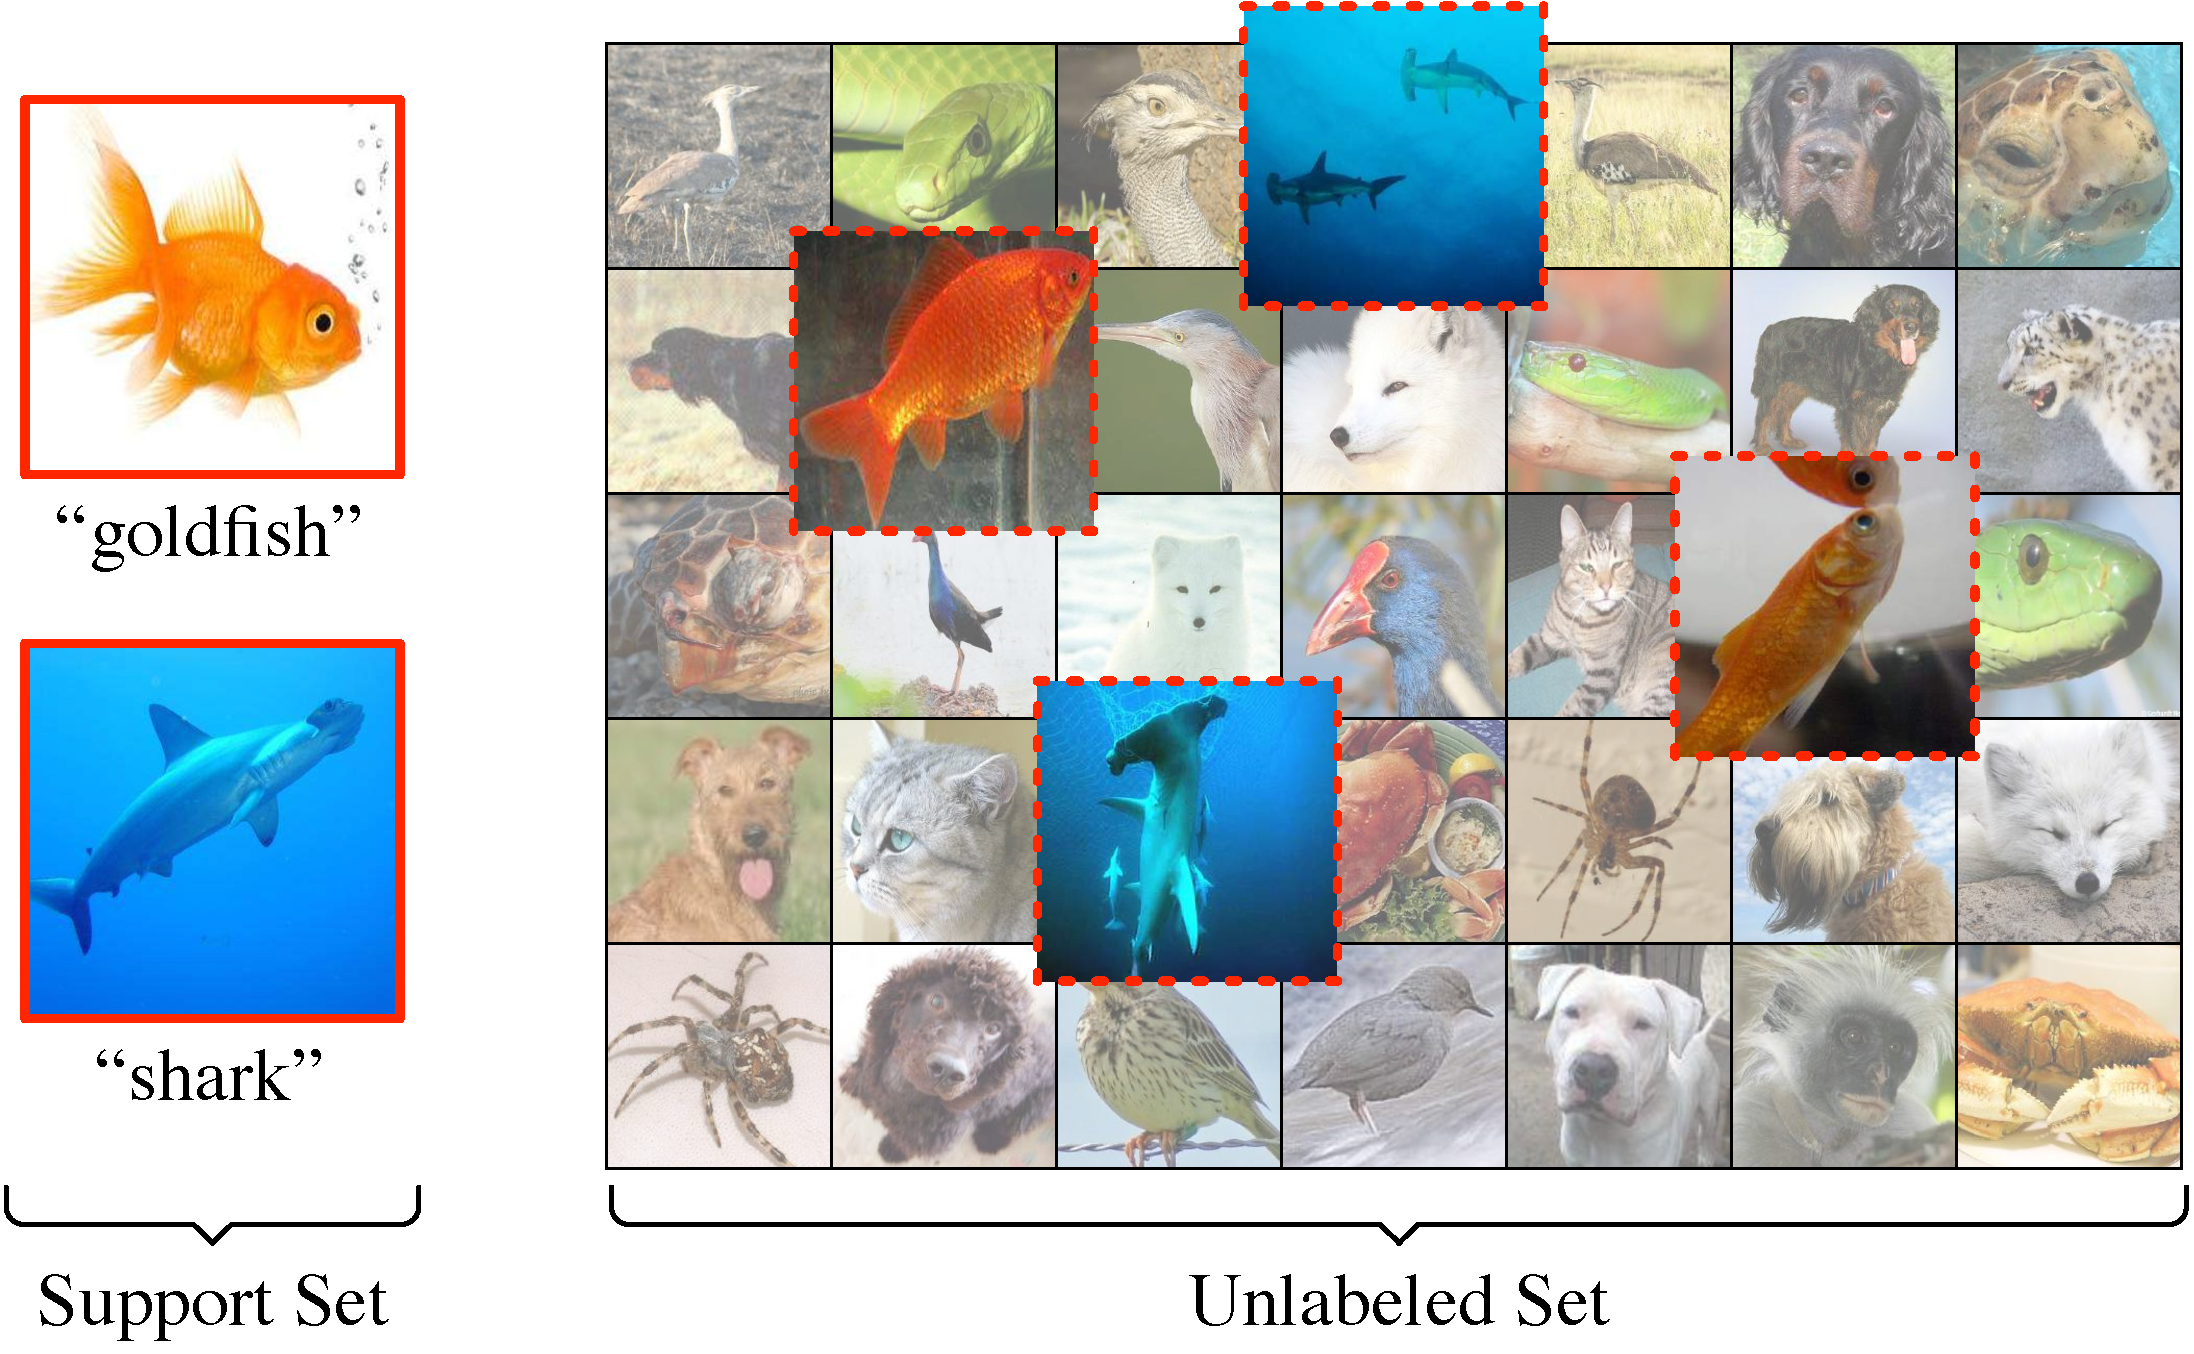
\includegraphics[width=0.48\textwidth]{figures/ssl_teaser_grid_distractor_fade_enlarge.pdf}
    \caption{Consider a setup where the aim is to learn a classifier to distinguish between two previously unseen classes, goldfish and shark, given not only labeled examples of these two classes, but also a larger pool of unlabeled examples, some of which may belong to one of these two classes of interest. %Specifically, we are exposed to a small number of labeled images for each of these two classes, denoted by a red border, and a larger number of unlabeled objects belonging to the classes of goldfish or shark, shown enlarged in this figure, as well as to ``background'' classes. 
    In this work we aim to move a step closer to this more natural learning framework by incorporating in our learning episodes unlabeled data from the classes we aim to learn representations for (shown with dashed red borders) as well as from {\it distractor} classes .}
    \label{fig:motivation}
    \vspace{-10pt}
\end{wrapfigure}
\fi